\documentclass[border=6pt,crop=true]{standalone}
\usepackage{pgfplots}
\pgfplotsset{compat=1.18}

\begin{document}
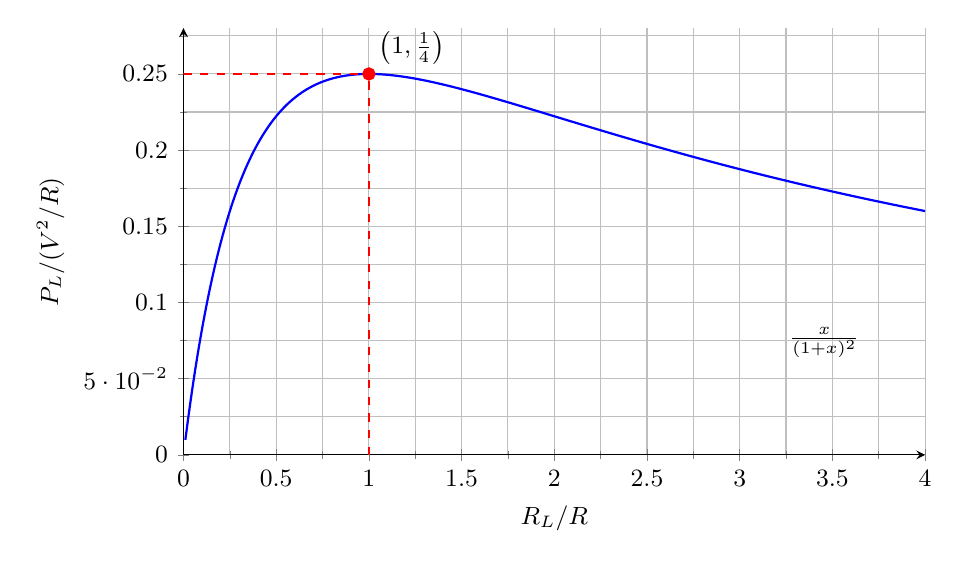
\begin{tikzpicture}
  \begin{axis}[
    width=11cm,
    height=7cm,
    axis lines=left,
    xlabel={$R_L / R$},
    ylabel={$P_L / (V^2 / R)$},
    xmin=0,
    xmax=4,
    ymin=0,
    ymax=0.28,
    domain=0.01:4,
    samples=300,
    grid=both,
    minor tick num=1,
    tick label style={font=\small},
    label style={font=\small},
    every axis plot/.append style={thick},
  ]
    \addplot[blue] {x/(1+x)^2};
    \addplot[red,dashed] coordinates {(1,0) (1,0.25)};
    \addplot[red,dashed] coordinates {(0,0.25) (1,0.25)};
    \addplot[mark=*,red] coordinates {(1,0.25)};

    \node[anchor=south west,font=\small] at (axis cs:1,0.25) {$\left(1,\frac{1}{4}\right)$};
    \node[anchor=north east,font=\small] at (axis cs:3.7,0.09) {$\frac{x}{(1+x)^2}$};
  \end{axis}
\end{tikzpicture}
\end{document}
